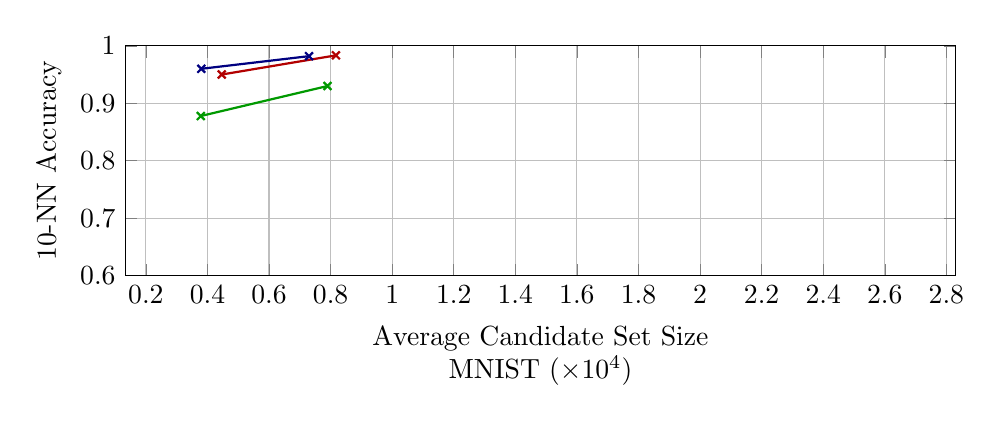
\begin{tikzpicture}
        \begin{axis}[
            width=\linewidth,
            height=4.5cm,
            grid=major,
            xlabel={\begin{tabular}{@{}c@{}}Average Candidate Set Size\\ MNIST ($\times 10^4$)\end{tabular}},
            ylabel={10-NN Accuracy},
            mark options={solid},
            xtick scale label code/.code={},
            xticklabel style={align=center},
            xmax=28299,
            ymin=0.6,
            ymax=1
        ]
        
        % Original
        \addplot[blue!50!black, thick, mark=x, mark size=2pt] coordinates {
            (3800, 0.96)
            (7300, 0.982)
        };
        % PCA
        \addplot[red!70!black, thick, mark=x, mark size=2pt] coordinates {
            (4465, 0.95)
            (8173, 0.9834)
        };
        % Mahalanobis
        \addplot[green!60!black, thick, mark=x, mark size=2pt] coordinates {
            (3784, 0.8778)
            (7899, 0.93)
        };
        \end{axis}
\end{tikzpicture}